\documentclass{article} % For LaTeX2e
\usepackage{iclr2024_conference,times}

% Stolen style files from ICLR 2024
% Optional math commands from https://github.com/goodfeli/dlbook_notation.
%%%%% NEW MATH DEFINITIONS %%%%%

\newcommand{\points}[1]{\texttt{\textbf{\textcolor{blue}{[#1 points]}}}}


\usepackage{amsmath,amsfonts,bm}

% Mark sections of captions for referring to divisions of figures
\newcommand{\figleft}{{\em (Left)}}
\newcommand{\figcenter}{{\em (Center)}}
\newcommand{\figright}{{\em (Right)}}
\newcommand{\figtop}{{\em (Top)}}
\newcommand{\figbottom}{{\em (Bottom)}}
\newcommand{\captiona}{{\em (a)}}
\newcommand{\captionb}{{\em (b)}}
\newcommand{\captionc}{{\em (c)}}
\newcommand{\captiond}{{\em (d)}}

% Highlight a newly defined term
\newcommand{\newterm}[1]{{\bf #1}}


% Figure reference, lower-case.
\def\figref#1{figure~\ref{#1}}
% Figure reference, capital. For start of sentence
\def\Figref#1{Figure~\ref{#1}}
\def\twofigref#1#2{figures \ref{#1} and \ref{#2}}
\def\quadfigref#1#2#3#4{figures \ref{#1}, \ref{#2}, \ref{#3} and \ref{#4}}
% Section reference, lower-case.
\def\secref#1{section~\ref{#1}}
% Section reference, capital.
\def\Secref#1{Section~\ref{#1}}
% Reference to two sections.
\def\twosecrefs#1#2{sections \ref{#1} and \ref{#2}}
% Reference to three sections.
\def\secrefs#1#2#3{sections \ref{#1}, \ref{#2} and \ref{#3}}
% Reference to an equation, lower-case.
\def\eqref#1{equation~\ref{#1}}
% Reference to an equation, upper case
\def\Eqref#1{Equation~\ref{#1}}
% A raw reference to an equation---avoid using if possible
\def\plaineqref#1{\ref{#1}}
% Reference to a chapter, lower-case.
\def\chapref#1{chapter~\ref{#1}}
% Reference to an equation, upper case.
\def\Chapref#1{Chapter~\ref{#1}}
% Reference to a range of chapters
\def\rangechapref#1#2{chapters\ref{#1}--\ref{#2}}
% Reference to an algorithm, lower-case.
\def\algref#1{algorithm~\ref{#1}}
% Reference to an algorithm, upper case.
\def\Algref#1{Algorithm~\ref{#1}}
\def\twoalgref#1#2{algorithms \ref{#1} and \ref{#2}}
\def\Twoalgref#1#2{Algorithms \ref{#1} and \ref{#2}}
% Reference to a part, lower case
\def\partref#1{part~\ref{#1}}
% Reference to a part, upper case
\def\Partref#1{Part~\ref{#1}}
\def\twopartref#1#2{parts \ref{#1} and \ref{#2}}

\def\ceil#1{\lceil #1 \rceil}
\def\floor#1{\lfloor #1 \rfloor}
\def\1{\bm{1}}
\newcommand{\train}{\mathcal{D}}
\newcommand{\valid}{\mathcal{D_{\mathrm{valid}}}}
\newcommand{\test}{\mathcal{D_{\mathrm{test}}}}

\def\eps{{\epsilon}}


% Random variables
\def\reta{{\textnormal{$\eta$}}}
\def\ra{{\textnormal{a}}}
\def\rb{{\textnormal{b}}}
\def\rc{{\textnormal{c}}}
\def\rd{{\textnormal{d}}}
\def\re{{\textnormal{e}}}
\def\rf{{\textnormal{f}}}
\def\rg{{\textnormal{g}}}
\def\rh{{\textnormal{h}}}
\def\ri{{\textnormal{i}}}
\def\rj{{\textnormal{j}}}
\def\rk{{\textnormal{k}}}
\def\rl{{\textnormal{l}}}
% rm is already a command, just don't name any random variables m
\def\rn{{\textnormal{n}}}
\def\ro{{\textnormal{o}}}
\def\rp{{\textnormal{p}}}
\def\rq{{\textnormal{q}}}
\def\rr{{\textnormal{r}}}
\def\rs{{\textnormal{s}}}
\def\rt{{\textnormal{t}}}
\def\ru{{\textnormal{u}}}
\def\rv{{\textnormal{v}}}
\def\rw{{\textnormal{w}}}
\def\rx{{\textnormal{x}}}
\def\ry{{\textnormal{y}}}
\def\rz{{\textnormal{z}}}

% Random vectors
\def\rvepsilon{{\mathbf{\epsilon}}}
\def\rvtheta{{\mathbf{\theta}}}
\def\rva{{\mathbf{a}}}
\def\rvb{{\mathbf{b}}}
\def\rvc{{\mathbf{c}}}
\def\rvd{{\mathbf{d}}}
\def\rve{{\mathbf{e}}}
\def\rvf{{\mathbf{f}}}
\def\rvg{{\mathbf{g}}}
\def\rvh{{\mathbf{h}}}
\def\rvu{{\mathbf{i}}}
\def\rvj{{\mathbf{j}}}
\def\rvk{{\mathbf{k}}}
\def\rvl{{\mathbf{l}}}
\def\rvm{{\mathbf{m}}}
\def\rvn{{\mathbf{n}}}
\def\rvo{{\mathbf{o}}}
\def\rvp{{\mathbf{p}}}
\def\rvq{{\mathbf{q}}}
\def\rvr{{\mathbf{r}}}
\def\rvs{{\mathbf{s}}}
\def\rvt{{\mathbf{t}}}
\def\rvu{{\mathbf{u}}}
\def\rvv{{\mathbf{v}}}
\def\rvw{{\mathbf{w}}}
\def\rvx{{\mathbf{x}}}
\def\rvy{{\mathbf{y}}}
\def\rvz{{\mathbf{z}}}

% Elements of random vectors
\def\erva{{\textnormal{a}}}
\def\ervb{{\textnormal{b}}}
\def\ervc{{\textnormal{c}}}
\def\ervd{{\textnormal{d}}}
\def\erve{{\textnormal{e}}}
\def\ervf{{\textnormal{f}}}
\def\ervg{{\textnormal{g}}}
\def\ervh{{\textnormal{h}}}
\def\ervi{{\textnormal{i}}}
\def\ervj{{\textnormal{j}}}
\def\ervk{{\textnormal{k}}}
\def\ervl{{\textnormal{l}}}
\def\ervm{{\textnormal{m}}}
\def\ervn{{\textnormal{n}}}
\def\ervo{{\textnormal{o}}}
\def\ervp{{\textnormal{p}}}
\def\ervq{{\textnormal{q}}}
\def\ervr{{\textnormal{r}}}
\def\ervs{{\textnormal{s}}}
\def\ervt{{\textnormal{t}}}
\def\ervu{{\textnormal{u}}}
\def\ervv{{\textnormal{v}}}
\def\ervw{{\textnormal{w}}}
\def\ervx{{\textnormal{x}}}
\def\ervy{{\textnormal{y}}}
\def\ervz{{\textnormal{z}}}

% Random matrices
\def\rmA{{\mathbf{A}}}
\def\rmB{{\mathbf{B}}}
\def\rmC{{\mathbf{C}}}
\def\rmD{{\mathbf{D}}}
\def\rmE{{\mathbf{E}}}
\def\rmF{{\mathbf{F}}}
\def\rmG{{\mathbf{G}}}
\def\rmH{{\mathbf{H}}}
\def\rmI{{\mathbf{I}}}
\def\rmJ{{\mathbf{J}}}
\def\rmK{{\mathbf{K}}}
\def\rmL{{\mathbf{L}}}
\def\rmM{{\mathbf{M}}}
\def\rmN{{\mathbf{N}}}
\def\rmO{{\mathbf{O}}}
\def\rmP{{\mathbf{P}}}
\def\rmQ{{\mathbf{Q}}}
\def\rmR{{\mathbf{R}}}
\def\rmS{{\mathbf{S}}}
\def\rmT{{\mathbf{T}}}
\def\rmU{{\mathbf{U}}}
\def\rmV{{\mathbf{V}}}
\def\rmW{{\mathbf{W}}}
\def\rmX{{\mathbf{X}}}
\def\rmY{{\mathbf{Y}}}
\def\rmZ{{\mathbf{Z}}}

% Elements of random matrices
\def\ermA{{\textnormal{A}}}
\def\ermB{{\textnormal{B}}}
\def\ermC{{\textnormal{C}}}
\def\ermD{{\textnormal{D}}}
\def\ermE{{\textnormal{E}}}
\def\ermF{{\textnormal{F}}}
\def\ermG{{\textnormal{G}}}
\def\ermH{{\textnormal{H}}}
\def\ermI{{\textnormal{I}}}
\def\ermJ{{\textnormal{J}}}
\def\ermK{{\textnormal{K}}}
\def\ermL{{\textnormal{L}}}
\def\ermM{{\textnormal{M}}}
\def\ermN{{\textnormal{N}}}
\def\ermO{{\textnormal{O}}}
\def\ermP{{\textnormal{P}}}
\def\ermQ{{\textnormal{Q}}}
\def\ermR{{\textnormal{R}}}
\def\ermS{{\textnormal{S}}}
\def\ermT{{\textnormal{T}}}
\def\ermU{{\textnormal{U}}}
\def\ermV{{\textnormal{V}}}
\def\ermW{{\textnormal{W}}}
\def\ermX{{\textnormal{X}}}
\def\ermY{{\textnormal{Y}}}
\def\ermZ{{\textnormal{Z}}}

% Vectors
\def\vzero{{\bm{0}}}
\def\vone{{\bm{1}}}
\def\vmu{{\bm{\mu}}}
\def\vtheta{{\bm{\theta}}}
\def\va{{\bm{a}}}
\def\vb{{\bm{b}}}
\def\vc{{\bm{c}}}
\def\vd{{\bm{d}}}
\def\ve{{\bm{e}}}
\def\vf{{\bm{f}}}
\def\vg{{\bm{g}}}
\def\vh{{\bm{h}}}
\def\vi{{\bm{i}}}
\def\vj{{\bm{j}}}
\def\vk{{\bm{k}}}
\def\vl{{\bm{l}}}
\def\vm{{\bm{m}}}
\def\vn{{\bm{n}}}
\def\vo{{\bm{o}}}
\def\vp{{\bm{p}}}
\def\vq{{\bm{q}}}
\def\vr{{\bm{r}}}
\def\vs{{\bm{s}}}
\def\vt{{\bm{t}}}
\def\vu{{\bm{u}}}
\def\vv{{\bm{v}}}
\def\vw{{\bm{w}}}
\def\vx{{\bm{x}}}
\def\vy{{\bm{y}}}
\def\vz{{\bm{z}}}

% Elements of vectors
\def\evalpha{{\alpha}}
\def\evbeta{{\beta}}
\def\evepsilon{{\epsilon}}
\def\evlambda{{\lambda}}
\def\evomega{{\omega}}
\def\evmu{{\mu}}
\def\evpsi{{\psi}}
\def\evsigma{{\sigma}}
\def\evtheta{{\theta}}
\def\eva{{a}}
\def\evb{{b}}
\def\evc{{c}}
\def\evd{{d}}
\def\eve{{e}}
\def\evf{{f}}
\def\evg{{g}}
\def\evh{{h}}
\def\evi{{i}}
\def\evj{{j}}
\def\evk{{k}}
\def\evl{{l}}
\def\evm{{m}}
\def\evn{{n}}
\def\evo{{o}}
\def\evp{{p}}
\def\evq{{q}}
\def\evr{{r}}
\def\evs{{s}}
\def\evt{{t}}
\def\evu{{u}}
\def\evv{{v}}
\def\evw{{w}}
\def\evx{{x}}
\def\evy{{y}}
\def\evz{{z}}

% Matrix
\def\mA{{\bm{A}}}
\def\mB{{\bm{B}}}
\def\mC{{\bm{C}}}
\def\mD{{\bm{D}}}
\def\mE{{\bm{E}}}
\def\mF{{\bm{F}}}
\def\mG{{\bm{G}}}
\def\mH{{\bm{H}}}
\def\mI{{\bm{I}}}
\def\mJ{{\bm{J}}}
\def\mK{{\bm{K}}}
\def\mL{{\bm{L}}}
\def\mM{{\bm{M}}}
\def\mN{{\bm{N}}}
\def\mO{{\bm{O}}}
\def\mP{{\bm{P}}}
\def\mQ{{\bm{Q}}}
\def\mR{{\bm{R}}}
\def\mS{{\bm{S}}}
\def\mT{{\bm{T}}}
\def\mU{{\bm{U}}}
\def\mV{{\bm{V}}}
\def\mW{{\bm{W}}}
\def\mX{{\bm{X}}}
\def\mY{{\bm{Y}}}
\def\mZ{{\bm{Z}}}
\def\mBeta{{\bm{\beta}}}
\def\mPhi{{\bm{\Phi}}}
\def\mLambda{{\bm{\Lambda}}}
\def\mSigma{{\bm{\Sigma}}}

% Tensor
\DeclareMathAlphabet{\mathsfit}{\encodingdefault}{\sfdefault}{m}{sl}
\SetMathAlphabet{\mathsfit}{bold}{\encodingdefault}{\sfdefault}{bx}{n}
\newcommand{\tens}[1]{\bm{\mathsfit{#1}}}
\def\tA{{\tens{A}}}
\def\tB{{\tens{B}}}
\def\tC{{\tens{C}}}
\def\tD{{\tens{D}}}
\def\tE{{\tens{E}}}
\def\tF{{\tens{F}}}
\def\tG{{\tens{G}}}
\def\tH{{\tens{H}}}
\def\tI{{\tens{I}}}
\def\tJ{{\tens{J}}}
\def\tK{{\tens{K}}}
\def\tL{{\tens{L}}}
\def\tM{{\tens{M}}}
\def\tN{{\tens{N}}}
\def\tO{{\tens{O}}}
\def\tP{{\tens{P}}}
\def\tQ{{\tens{Q}}}
\def\tR{{\tens{R}}}
\def\tS{{\tens{S}}}
\def\tT{{\tens{T}}}
\def\tU{{\tens{U}}}
\def\tV{{\tens{V}}}
\def\tW{{\tens{W}}}
\def\tX{{\tens{X}}}
\def\tY{{\tens{Y}}}
\def\tZ{{\tens{Z}}}


% Graph
\def\gA{{\mathcal{A}}}
\def\gB{{\mathcal{B}}}
\def\gC{{\mathcal{C}}}
\def\gD{{\mathcal{D}}}
\def\gE{{\mathcal{E}}}
\def\gF{{\mathcal{F}}}
\def\gG{{\mathcal{G}}}
\def\gH{{\mathcal{H}}}
\def\gI{{\mathcal{I}}}
\def\gJ{{\mathcal{J}}}
\def\gK{{\mathcal{K}}}
\def\gL{{\mathcal{L}}}
\def\gM{{\mathcal{M}}}
\def\gN{{\mathcal{N}}}
\def\gO{{\mathcal{O}}}
\def\gP{{\mathcal{P}}}
\def\gQ{{\mathcal{Q}}}
\def\gR{{\mathcal{R}}}
\def\gS{{\mathcal{S}}}
\def\gT{{\mathcal{T}}}
\def\gU{{\mathcal{U}}}
\def\gV{{\mathcal{V}}}
\def\gW{{\mathcal{W}}}
\def\gX{{\mathcal{X}}}
\def\gY{{\mathcal{Y}}}
\def\gZ{{\mathcal{Z}}}

% Sets
\def\sA{{\mathbb{A}}}
\def\sB{{\mathbb{B}}}
\def\sC{{\mathbb{C}}}
\def\sD{{\mathbb{D}}}
% Don't use a set called E, because this would be the same as our symbol
% for expectation.
\def\sF{{\mathbb{F}}}
\def\sG{{\mathbb{G}}}
\def\sH{{\mathbb{H}}}
\def\sI{{\mathbb{I}}}
\def\sJ{{\mathbb{J}}}
\def\sK{{\mathbb{K}}}
\def\sL{{\mathbb{L}}}
\def\sM{{\mathbb{M}}}
\def\sN{{\mathbb{N}}}
\def\sO{{\mathbb{O}}}
\def\sP{{\mathbb{P}}}
\def\sQ{{\mathbb{Q}}}
\def\sR{{\mathbb{R}}}
\def\sS{{\mathbb{S}}}
\def\sT{{\mathbb{T}}}
\def\sU{{\mathbb{U}}}
\def\sV{{\mathbb{V}}}
\def\sW{{\mathbb{W}}}
\def\sX{{\mathbb{X}}}
\def\sY{{\mathbb{Y}}}
\def\sZ{{\mathbb{Z}}}

% Entries of a matrix
\def\emLambda{{\Lambda}}
\def\emA{{A}}
\def\emB{{B}}
\def\emC{{C}}
\def\emD{{D}}
\def\emE{{E}}
\def\emF{{F}}
\def\emG{{G}}
\def\emH{{H}}
\def\emI{{I}}
\def\emJ{{J}}
\def\emK{{K}}
\def\emL{{L}}
\def\emM{{M}}
\def\emN{{N}}
\def\emO{{O}}
\def\emP{{P}}
\def\emQ{{Q}}
\def\emR{{R}}
\def\emS{{S}}
\def\emT{{T}}
\def\emU{{U}}
\def\emV{{V}}
\def\emW{{W}}
\def\emX{{X}}
\def\emY{{Y}}
\def\emZ{{Z}}
\def\emSigma{{\Sigma}}

% entries of a tensor
% Same font as tensor, without \bm wrapper
\newcommand{\etens}[1]{\mathsfit{#1}}
\def\etLambda{{\etens{\Lambda}}}
\def\etA{{\etens{A}}}
\def\etB{{\etens{B}}}
\def\etC{{\etens{C}}}
\def\etD{{\etens{D}}}
\def\etE{{\etens{E}}}
\def\etF{{\etens{F}}}
\def\etG{{\etens{G}}}
\def\etH{{\etens{H}}}
\def\etI{{\etens{I}}}
\def\etJ{{\etens{J}}}
\def\etK{{\etens{K}}}
\def\etL{{\etens{L}}}
\def\etM{{\etens{M}}}
\def\etN{{\etens{N}}}
\def\etO{{\etens{O}}}
\def\etP{{\etens{P}}}
\def\etQ{{\etens{Q}}}
\def\etR{{\etens{R}}}
\def\etS{{\etens{S}}}
\def\etT{{\etens{T}}}
\def\etU{{\etens{U}}}
\def\etV{{\etens{V}}}
\def\etW{{\etens{W}}}
\def\etX{{\etens{X}}}
\def\etY{{\etens{Y}}}
\def\etZ{{\etens{Z}}}

% The true underlying data generating distribution
\newcommand{\pdata}{p_{\rm{data}}}
% The empirical distribution defined by the training set
\newcommand{\ptrain}{\hat{p}_{\rm{data}}}
\newcommand{\Ptrain}{\hat{P}_{\rm{data}}}
% The model distribution
\newcommand{\pmodel}{p_{\rm{model}}}
\newcommand{\Pmodel}{P_{\rm{model}}}
\newcommand{\ptildemodel}{\tilde{p}_{\rm{model}}}
% Stochastic autoencoder distributions
\newcommand{\pencode}{p_{\rm{encoder}}}
\newcommand{\pdecode}{p_{\rm{decoder}}}
\newcommand{\precons}{p_{\rm{reconstruct}}}

\newcommand{\laplace}{\mathrm{Laplace}} % Laplace distribution

\newcommand{\E}{\mathbb{E}}
\newcommand{\Ls}{\mathcal{L}}
\newcommand{\R}{\mathbb{R}}
\newcommand{\emp}{\tilde{p}}
\newcommand{\lr}{\alpha}
\newcommand{\reg}{\lambda}
\newcommand{\rect}{\mathrm{rectifier}}
\newcommand{\softmax}{\mathrm{softmax}}
\newcommand{\sigmoid}{\sigma}
\newcommand{\softplus}{\zeta}
\newcommand{\KL}{D_{\mathrm{KL}}}
\newcommand{\Var}{\mathrm{Var}}
\newcommand{\standarderror}{\mathrm{SE}}
\newcommand{\Cov}{\mathrm{Cov}}
% Wolfram Mathworld says $L^2$ is for function spaces and $\ell^2$ is for vectors
% But then they seem to use $L^2$ for vectors throughout the site, and so does
% wikipedia.
\newcommand{\normlzero}{L^0}
\newcommand{\normlone}{L^1}
\newcommand{\normltwo}{L^2}
\newcommand{\normlp}{L^p}
\newcommand{\normmax}{L^\infty}

\newcommand{\parents}{Pa} % See usage in notation.tex. Chosen to match Daphne's book.

\DeclareMathOperator*{\argmax}{arg\,max}
\DeclareMathOperator*{\argmin}{arg\,min}

\DeclareMathOperator{\sign}{sign}
\DeclareMathOperator{\Tr}{Tr}
\let\ab\allowbreak


\usepackage{hyperref}
\usepackage{url}
\usepackage{graphicx}
\usepackage{booktabs}
\usepackage{multirow}
\usepackage{float}

\iclrfinalcopy

\title{MD4AD: Dataset Proposal and Analysis}

\author{
	Daniel Yang\thanks{\hspace{4pt}Everyone Contributed Equally -- Alphabetical order} \hspace{2em} Junhong Zhou$^*$ \hspace{2em} Patrick Chen$^*$ \hspace{2em} Tianzhi Li $^*$ \\
	\texttt{\{danielya, junhong2, bochunc, tianzhil\}@andrew.cmu.edu}
}


\date{}

\begin{document}
	\maketitle
	
	\section{\points{4} Problem Definition and Dataset Choice}
	%Include paper title, link to data, etc.  If you are creating something, provide details about the process and basis.
	%If you are choosing a dataset not listed on the course website, this section should be long enough to justify that you are qualified for your choice.  This may mean a second page.
	
	\subsection*{Problem Definition}
	\begin{figure}[H]
		\centering
		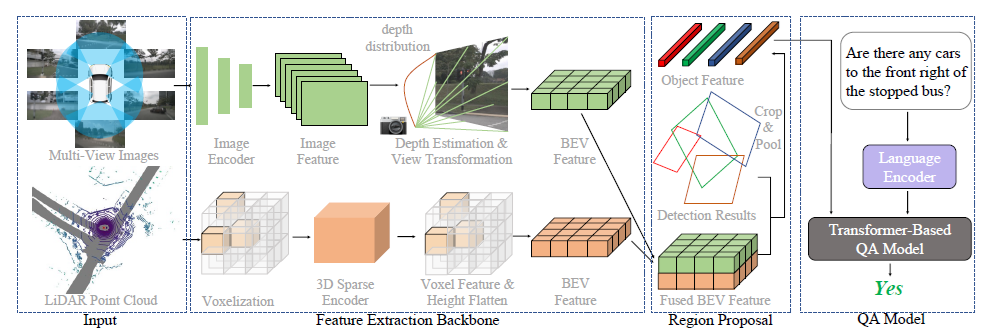
\includegraphics[width=0.9\textwidth]{./Figures/Baseline_Framework.png}
		\caption{Baseline Framework \cite{qian2024nuscenes}.}
		\label{fig:framework}
	\end{figure}
	
	We aim to improve \textbf{visual question answering (VQA) in the autonomous driving domain} by enhancing the baseline model of \textbf{NuScenes-QA}~\cite{qian2024nuscenes} with \href{https://github.com/taco-group/OpenEMMA}{\textbf{Open Emma}}~\cite{openemma}, an advanced QA model. Our work is based on the paper \textit{NuScenes-QA: A Multi-Modal Visual Question Answering Benchmark for Autonomous Driving Scenario} by Tianwen Qian et al.~\cite{qian2024nuscenes}, which introduces a novel benchmark for VQA in autonomous driving. As above \autoref{fig:framework} in the paper, our goal is to replace the existing QA model with \textbf{Open EMMA} while ensuring that the outputs align with the \textbf{ground truth} and \textbf{NuScenes-QA question-answering context} through a carefully designed \textbf{loss function}.
	
	Additionally, we propose to \textbf{replace the feature extraction backbone} and \textbf{region proposal module} with \textbf{more advanced vision and LiDAR encoders}. We also explore the integration of \textbf{knowledge graphs or scene graphs (or both)} to improve spatial reasoning and object relationship understanding. This enhanced framework aims to \textbf{achieve higher accuracy and better generalization} in the NuScenes-QA benchmark.
	
	\subsection*{Dataset Choice}
	We utilize \textbf{NuScenes-QA}, a large-scale \textbf{multi-modal visual question answering dataset} specifically designed for \textbf{autonomous driving}. This dataset is built upon \textbf{NuScenes}, a widely used \textbf{3D perception dataset}, and contains:
	\begin{itemize}
		\item \textbf{34,000+ driving scenes}
		\item \textbf{450,000+ question-answer pairs}
		\item \textbf{Multi-modal inputs}: multi-view images, LiDAR point clouds, and text (QA pairs)
		\item \textbf{Diverse question types}: existence, counting, object query, object-status query, and comparison
	\end{itemize}
	
	The NuScenes-QA dataset and related resources can be accessed at \url{https://github.com/qiantianwen/NuScenes-QA}.
	
	Compared to existing VQA benchmarks, NuScenes-QA introduces new challenges, such as \textbf{multi-frame temporal reasoning}, \textbf{multi-modal sensor fusion}, and \textbf{dynamic scene understanding}. These challenges make it an ideal dataset for evaluating the effectiveness of our proposed modifications.
	
	\subsection{\points{0.5} What phenomena or task does this dataset help address?}
	The NuScenes-QA dataset helps address \textbf{visual question answering (VQA) task for autonomous driving}, enabling models to understand \textbf{spatial status, object interactions, and temporal events in dynamic traffic environments}. The dataset provides \textbf{multi-modal data} (multi-view images, LiDAR, and text QA pairs) to improve perception-based question answering, making it useful for tasks like \textbf{scene understanding, object detection, and reasoning in complex urban scenarios}.
	
	
	\subsection{\points{0.5}  What about this task is fundamentally multimodal?}
	This task is fundamentally multimodal because \textbf{it requires integrating multiple sensor modalities}—RGB images and LiDAR point clouds—to sense the environment, and joint learning with language input (text) to \textbf{derive meaningful answers}. Questions often require \textbf{correlating spatial and depth information} from different perspectives, making it insufficient to rely on a single modality. For example, a question like ``What is the distance between the red car and the pedestrian?" requires using \textbf{RGB images} for color detection and \textbf{LiDAR point clouds} for precise depth estimation. The dataset is designed in such a way that \textbf{cross-modal reasoning} is required, where \textbf{vision, language, and 3D spatial information} collectively contribute to accurate question answering.
	
	\subsection{Hypotheses}
	
	\paragraph{\points{1} Hypothesis}
	
	\textbf{Fusion of camera and LiDAR data improves object recognition in complex driving environments.}
	
	We hypothesize that by combining camera images and LiDAR point clouds, we can significantly improve the accuracy of object recognition in the autonomous driving setting. The camera data provides rich visual details, while LiDAR offers precise depth information, especially in challenging environments like night driving or adverse weather conditions. This hypothesis will be tested by measuring the improvement in object detection accuracy when both modalities are used together, compared to using camera data or LiDAR data individually in the NuScenes-QA dataset.
	
	
	\paragraph{\points{1} Hypothesis}
	\textbf{Scene graphs enhance object relationship understanding in question answering.}
	
	We hypothesize that scene graphs improve the understanding of object relationships by explicitly linking visual data (e.g., images and LiDAR point clouds) with natural language, enhancing the accuracy of question answering in autonomous driving. Scene graphs provide a structured and semantically rich representation of the environment, allowing the model to better grasp spatial and relational connections between objects (e.g., ``car is near pedestrian," ``traffic light is ahead of vehicle"). This explicit representation helps the model answer complex questions by leveraging object relationships, such as  ``What is the distance to the nearest traffic sign?” The hypothesis will be tested by comparing question-answering models that utilize scene graphs for reasoning with those that process raw sensor data directly, assessing how scene graphs improve the model’s ability to understand and reason about object relationships in the NuScenes-QA dataset.
	
	% This criterion is linked to a Learning OutcomeHypothesis
	% 3 points total. For each of 3 hypotheses:
	% - 1/3 point: wrote something
	% - 1/3 point: specific to this task/dataset (not generically true of any multimodal dataset)
	% - 1/3 point: implies some actionable thing to test or model
	
	% \textbf{Scene graphs as a bridge between vision and language enhance the interpretability and explainability of question answering systems.}
	% We hypothesize that scene graphs, by acting as an intermediary between visual data (e.g., images and LiDAR point clouds) and natural language, improve the interpretability and explainability of question-answering models in autonomous driving. Scene graphs provide a structured and semantically rich representation of the environment, enabling the model to better understand the relationships between objects (e.g., "car is near pedestrian," "traffic light is ahead of vehicle"). By leveraging these connections, the QA system can offer more transparent and reasoned answers that are easily traceable to specific visual elements. This hypothesis will be tested by comparing question-answering models that use scene graphs for intermediate reasoning with models that process raw sensor data directly, assessing how scene graphs enhance the model's ability to explain its reasoning process and answer questions more coherently.
	
	
	
	
	% \paragraph{\points{1} Hypothesis}
	% \textbf{Scene graphs improve cross-modal reasoning by explicitly linking vision and language for fine-grained question answering.}
	% We hypothesize that scene graphs enable more effective cross-modal reasoning by explicitly linking visual features with linguistic components, thereby improving the accuracy and precision of fine-grained question answering in autonomous driving. Scene graphs create explicit associations between objects, their properties, and their spatial relations, making it easier for the QA system to connect specific details from the image (e.g., "stop sign," "pedestrian") with corresponding linguistic elements in the question. For instance, a question like “What is the distance to the nearest traffic sign?” can be answered more precisely when the model understands the exact spatial relationships between objects in the scene. This hypothesis will be tested by evaluating the performance of question-answering models on tasks that require fine-grained spatial and relational understanding, comparing models that utilize scene graphs versus those that rely solely on visual or textual features.
	
	\paragraph{\points{1}Hypothesis}
	\textbf{Incorporating knowledge graphs enhances spatial reasoning ability in driving-related question answering.}
	
	We hypothesize that by integrating knowledge graphs into the question-answering process, the model will improve its ability to reason about spatial relationships and interactions between objects, which is crucial for One-Hop (H1) questions in the NuScenes-QA dataset. These questions require the model to understand the positioning, movement, or proximity of objects in the scene, such as determining which vehicle is ahead of another or how far apart two objects are. Knowledge graphs can provide structured, relational information about object types, spatial constraints, and dynamic behaviors that are difficult to infer from RGB and LiDAR data alone. This hypothesis will be tested by measuring the model’s performance on One-Hop questions with and without the use of a knowledge graph, focusing on spatial reasoning tasks like identifying object relationships or predicting object trajectories in the NuScenes-QA dataset.
	
	% speed estimation
	% 运动物体的检测 & 速度估计
	
	
	\clearpage
	\section{\points{6} Dataset Analysis }
	\subsection{ \points{1} Dataset properties} 
	The \textbf{NuScenes-QA} dataset is designed to support visual question answering (VQA) in autonomous driving scenarios. It integrates multiple data modalities, including images, LiDAR point clouds, and rich annotations for comprehensive scene understanding. Key properties of the dataset include:
	
	\begin{itemize}
		\item \textbf{Dataset Size:} Over \textbf{34,000 driving scenes} and \textbf{450,000 question-answer pairs} under diverse urban environments.
		\item \textbf{Storage Size:} Approximately \textbf{1.4 TB} of data, including sensor data, annotations, and metadata.
		\item \textbf{Framerate:} Sensor data captured at \textbf{2 Hz} for LiDAR and \textbf{12 Hz} for cameras.
		\item \textbf{Physical Hardware Platform:} Collected using a \textbf{full-scale autonomous vehicle platform} equipped with \textbf{six cameras}, \textbf{five radars}, and \textbf{one 32-beam LiDAR sensor}.
		\item \textbf{Modalities:} Multi-modal inputs including \textbf{multi-view RGB images}, \textbf{LiDAR point clouds}, \textbf{radar data}, and \textbf{text of Question-Answering pairs}.
		\item \textbf{Annotation Types:} Detailed annotations with \textbf{3D bounding boxes}, \textbf{object categories}, \textbf{tracking IDs}, and \textbf{semantic maps} to support complex reasoning tasks.
		\item \textbf{Question Types:} A diverse set of question formats such as \textbf{existence}, \textbf{counting}, \textbf{object recognition}, \textbf{status analysis}, and \textbf{comparison} questions.
		\item \textbf{Class Distribution:} The dataset contains a total of 23 object classes, with the majority being \textbf{car} objects, followed by \textbf{adult} and \textbf{barrier} objects. This distribution highlights a noticeable class imbalance within the dataset.    
		\item \textbf{Temporal Sequences:} Multi-frame sequences for analyzing \textbf{temporal dynamics} and \textbf{object motion}.
		\item \textbf{Scene Complexity:} Includes diverse driving scenarios with varying \textbf{weather conditions}, \textbf{lighting}, and \textbf{traffic densities}, reflecting real-world autonomous driving environments.
	\end{itemize}
	
	\subsection{ \points{0.5} Compute Requirements}
	\begin{enumerate}
		\item Files (can fit in RAM?)
		%The Waymo Open Motion Dataset (WOMD) comprises over 100,000 segments, each 20 seconds long at a 10 Hz sampling rate, resulting in more than 570 hours of data and exceeding 1 TB in total size. The full dataset is too large to fit into RAM for typical workstations. However, it can be processed in smaller batches or individual segments, depending on the available memory. High-performance machines with large RAM capacities may handle more extensive portions of the dataset in memory, but for most use cases, data streaming or chunk-wise processing will be necessary.
		The nuScenes dataset is relatively large (around 1.4TB in total), which generally exceeds typical RAM capacities (e.g., 32GB or 64GB) of standard workstations. Consequently, most workflows involve storing the dataset on a local or network drive and loading subsets of the data into memory as needed (e.g., mini-batch loading during training). We will store the data in the server and using batch processing to retrieve the data while training.
		
		
		\item Models (can fit on GCP/AWS GPUs?)
		%Baseline models provided for WOMD are designed to be compatible with common cloud GPU platforms like GCP and AWS. These models like Emma\cite{Hwang2024EMMAEM} can be trained and deployed on GPUs such as NVIDIA Tesla V100, A100, or T4, which are available on GCP and AWS. The computational demands will vary depending on the model complexity and batch size, but standard GPU instances should suffice for training and inference tasks related to WOMD.
		Based on our analysis, we plan to use OpenEMMA with Llama-3.2-11B-Vision-Instruct (nearly 44GB) as our target model and fine-tune it using our four NVIDIA A6000 GPUs. Each A6000 provides 48GB of VRAM, giving us a total of 192GB, which should be sufficient to handle the memory demands of an 11-billion-parameter model. This setup allows us to distribute the computational load effectively across the GPUs, ensuring efficient training and fine-tuning. Compared to cloud-based GPU instances on platforms like GCP or AWS, our local configuration offers a cost-effective solution, provided we optimize the fine-tuning process to fully leverage multi-GPU parallelism and manage memory efficiently.
	\end{enumerate}
	\subsection{\points{2} Modality analysis}
	Using a small sample of the data (e.g. validation splits), generate statistics and plots for three relevant properties of the data.  
	
	\begin{enumerate}
		\item QA Paring Texts Analysis (\autoref{fig:QA}):
		\begin{figure}[H]
			\centering
			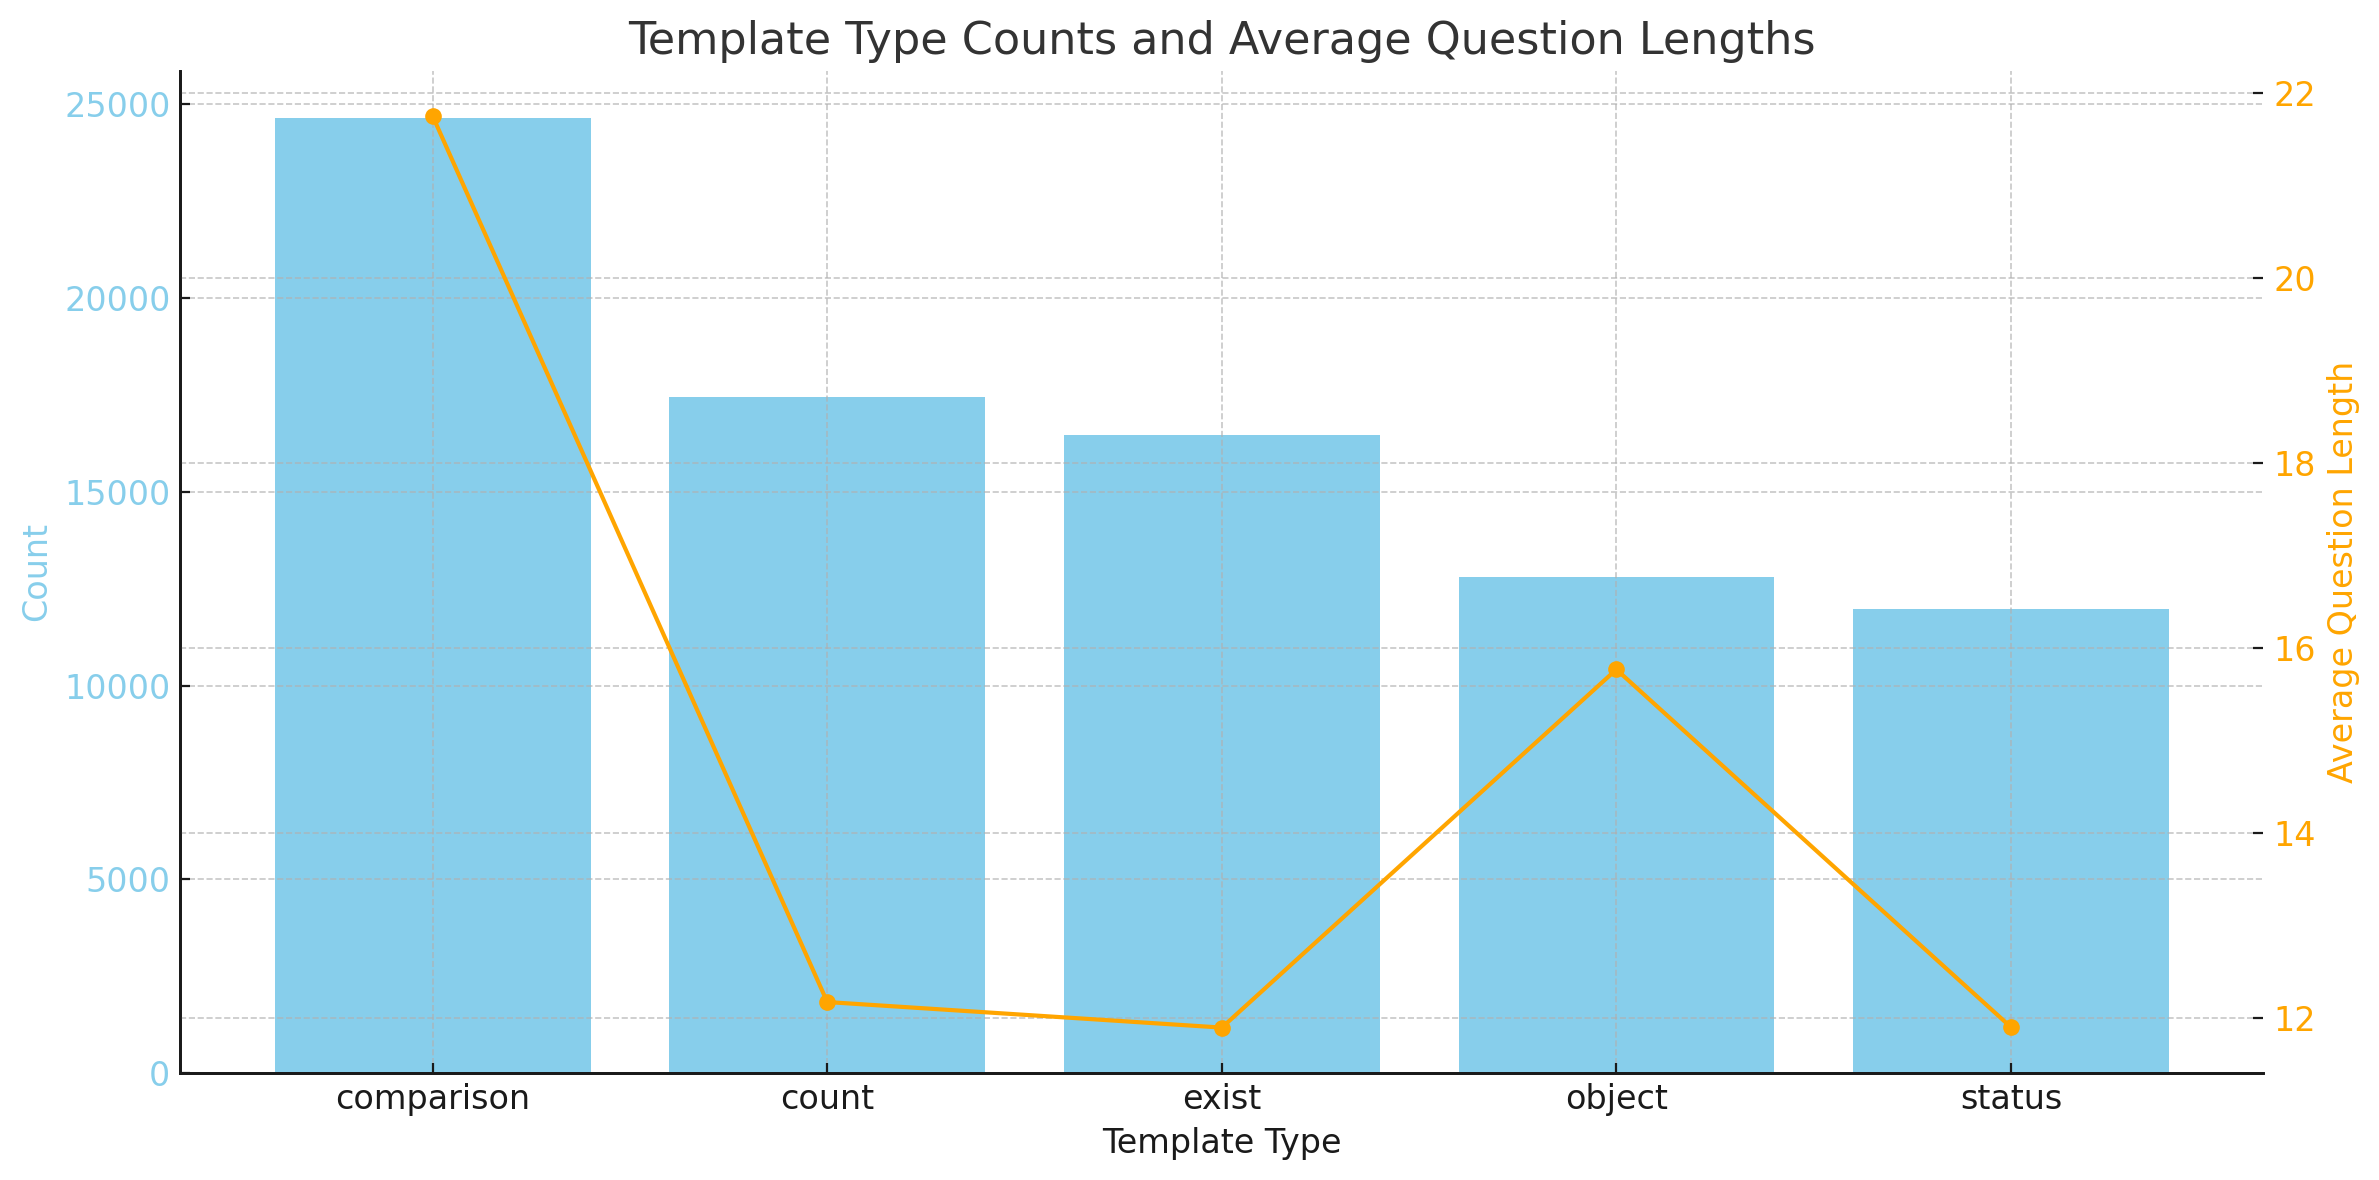
\includegraphics[width=0.9\textwidth]{Figures/Template Type Counts and Average Question Lengths.png}
			\caption{The bar chart represents the count of questions for each template type from NuScenes-QA, shown in blue. The orange line illustrates the average length of questions (in words) for each template type.}
			\label{fig:QA}
		\end{figure}
		\item Category Distribution (\autoref{fig:CD})
		\begin{figure}[H]
			\centering
			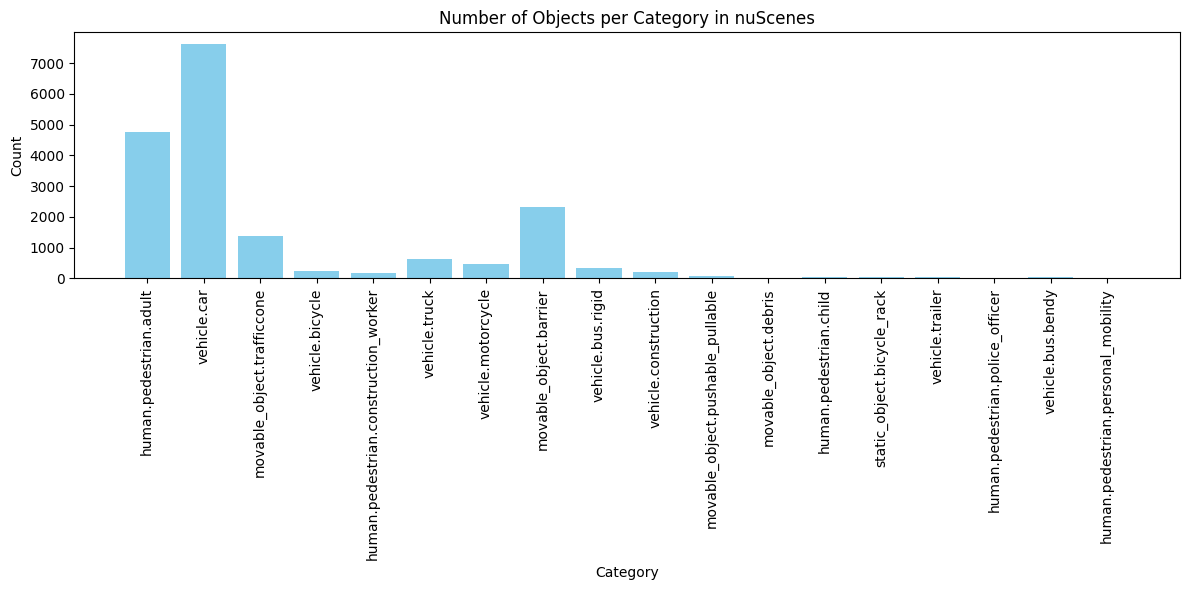
\includegraphics[width=0.9\textwidth]{Figures/nuscenes_category.png}
			\caption{This bar chart illustrates the distribution of object categories in the nuScenes mini dataset. Each bar represents the total number of annotated instances for a specific category, such as vehicles, pedestrians, and movable objects.}
			\label{fig:CD}
		\end{figure}
		\item Distribution of Bounding Boxes per Scene (\autoref{fig:ANBB})
		\begin{figure}[H]
			\centering
			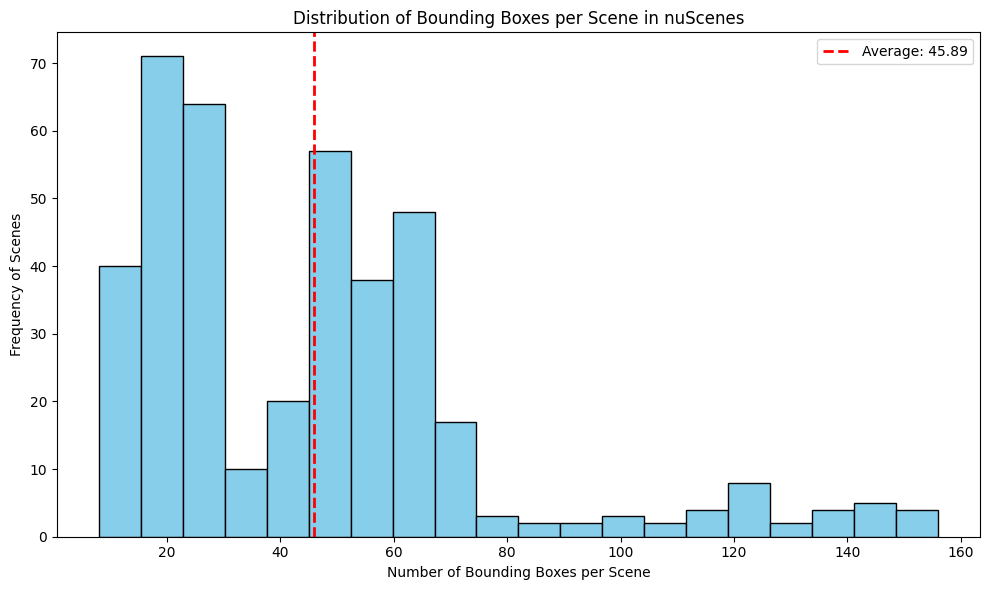
\includegraphics[width=0.9\textwidth]{./Figures/nuscenes_Frequency_of_Scenes.png}
			\caption{This histogram illustrates the distribution of bounding boxes per scene in the nuScenes mini dataset. The x-axis represents the number of bounding boxes in a scene, while the y-axis indicates the frequency of the scene with that number of bounding boxes. The red dashed line marks the average number of bounding boxes per scene.}
			\label{fig:ANBB}
		\end{figure}
		\item Number of Objects per Scene (\autoref{fig:NBI})
		\begin{figure}[H]
			\centering
			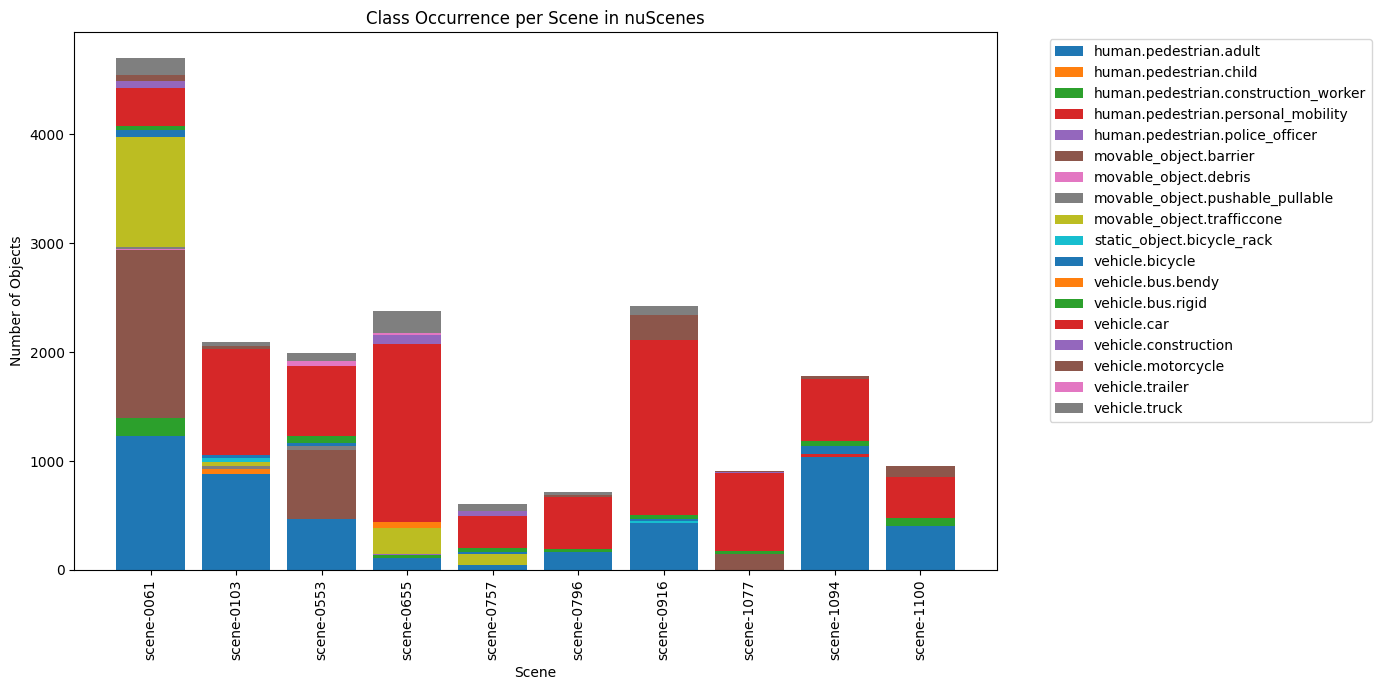
\includegraphics[width=0.9\textwidth]{Figures/nuscenes_class_occurrence.png}
			\caption{This stacked bar chart illustrates the distribution of object classes across different scenes in the nuScenes mini dataset. Each bar represents a scene, with colored segments indicating the number of occurrences of various object categories, such as vehicles, pedestrians, and movable objects.}
			\label{fig:NBI}
		\end{figure}
		\item Location and Date Distribution Visualization (\autoref{fig:LDDV})
		\begin{figure}[H]
			\centering
			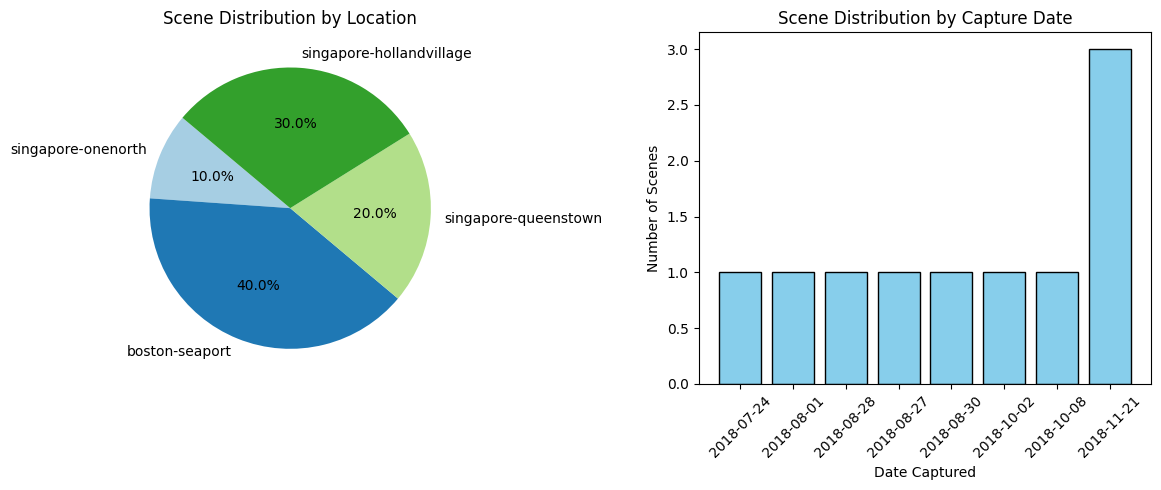
\includegraphics[width=0.9\textwidth]{Figures/Nuscenes_Location_and_Date_Distribution_Visualization.png}
			\caption{The pie chart illustrates the distribution of scenes across different locations in the nuScenes mini dataset, such as ‘Singapore’ or ‘Boston’. The bar graph shows the number of scenes captured on different dates.}
			\label{fig:LDDV}
		\end{figure}
		
		
		
		%\item The following \autoref{fig:class_dist} shows the class distribution in nuScenes dataset.
		%\begin{figure}[H] % Use [H] to force the figure to stay here
		%\centering
		%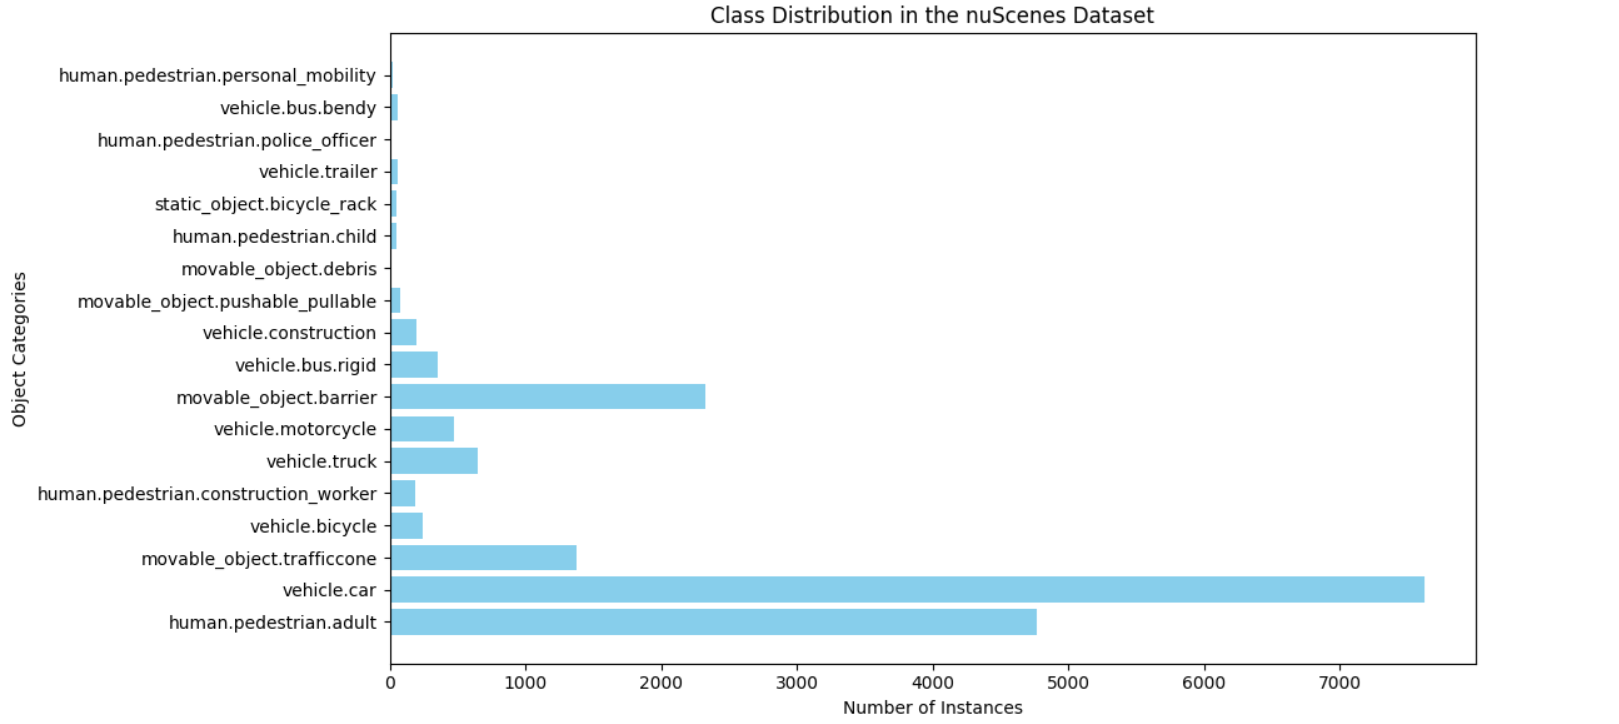
\includegraphics[width=0.9\textwidth]{./Figures/Obj_Dist.png}
		%\caption{Class Distribution}
		%\label{fig:class_dist}
		%\end{figure}    
		% \item Lexical diversity, sentence length, ...
		% \item Average number of objects detected per image
		% \item Degrees of freedom, number of articulated objects, ...
	\end{enumerate}
	\subsection{ \points{0.5} Metrics used}
	The primary evaluation metric used in NuScenes-QA is \textbf{Top-1 Accuracy}, which measures the proportion of correctly predicted answers out of the total number of questions. The accuracy is reported across different \textbf{question categories} and \textbf{reasoning complexities}, including:
	\begin{itemize}
		\item \textbf{Existence (Exist)}: Checks whether specific objects exist in the scene.
		\item \textbf{Counting (Count)}: Evaluates the model's ability to count objects meeting certain criteria.
		\item \textbf{Object Recognition (Object)}: Measures the accuracy of identifying specific objects based on descriptions.
		\item \textbf{Status Recognition (Status)}: Assesses the model's ability to determine the status (e.g., moving, parked) of objects.
		\item \textbf{Comparison (Comparison)}: Evaluates the model’s performance in comparing attributes between objects.
	\end{itemize}
	
	Additionally, the dataset distinguishes between:
	\begin{itemize}
		\item \textbf{Zero-Hop (H0)}: Questions that require no complex reasoning across objects.
		\item \textbf{One-Hop (H1)}: Questions that involve spatial reasoning or relationships between objects.
	\end{itemize}
	
	The accuracy is calculated for both \textbf{H0 and H1 separately} and then averaged to report the overall performance.
	
	
	\subsection{\points{2} Baselines} 
	
	The following baselines are all listed in the benchmark in nuScenes-QA paper \cite{qian2024nuscenes}
	
	\begin{itemize}
		\item \textbf{Q-Only Baseline}: This baseline model only considers the question text without using any visual input. It helps to understand how much language biases contribute to the performance. Although it performs decently for simple existence questions, it struggles with more complex reasoning tasks due to the absence of visual context.
		
		\item \textbf{BEVDet + BUTD (Bottom-Up and Top-Down Attention)}: This model combines BEVDet \cite{huang2021bevdet}, which processes multi-camera images to generate Bird’s Eye View (BEV) features, with the BUTD attention mechanism \cite{anderson2018bottom}. It improves performance by focusing on salient regions in the images. This combination is effective for object recognition tasks but struggles with complex reasoning due to limited LiDAR integration.
		
		\item \textbf{CenterPoint + MCAN (Modular Co-Attention Network)}: CenterPoint \cite{yin2021centerpoint} uses LiDAR data for precise 3D object detection, while MCAN \cite{yu2019deep} handles the interaction between visual and textual features through attention mechanisms. This model shows improved performance for spatial reasoning tasks, leveraging LiDAR’s strength in capturing structural information.
		
		\item \textbf{MSMDFusion + MCAN}: This is the strongest baseline, fusing multi-scale features from both LiDAR and camera data (MSMDFusion) \cite{zhang2022msmdfusion} and utilizing MCAN \cite{yu2019deep} for advanced feature interaction. The fusion approach significantly boosts performance by exploiting complementary information from different modalities, especially for tasks like comparison and status recognition.
	\end{itemize}
	\begin{table}[ht]
		\centering
		\resizebox{\textwidth}{!}{%
			\begin{tabular}{lcccccccccccccccc}
				\toprule
				\textbf{Models} & \multicolumn{3}{c}{\textbf{Exist}} & \multicolumn{3}{c}{\textbf{Count}} & \multicolumn{3}{c}{\textbf{Object}} & \multicolumn{3}{c}{\textbf{Status}} & \multicolumn{3}{c}{\textbf{Comparison}} & \textbf{Acc} \\
				\cmidrule(lr){2-4} \cmidrule(lr){5-7} \cmidrule(lr){8-10} \cmidrule(lr){11-13} \cmidrule(lr){14-16}
				& H0 & H1 & All & H0 & H1 & All & H0 & H1 & All & H0 & H1 & All & H0 & H1 & All  \\
				\midrule
				Q-Only               & 81.7 & 77.9 & 79.6 & 17.8 & 16.5 & 17.2 & 59.4 & 38.9 & 42.0 & 57.2 & 48.3 & 51.3 & 79.5 & 65.7 & 66.9 & 53.4 \\
				\midrule
				BEVDet+BUTD          & 87.2 & 80.6 & 83.7 & 21.7 & 20.0 & 20.9 & 69.4 & 45.2 & 48.8 & 55.0 & 50.5 & 52.0 & 76.1 & 66.8 & 67.6 & 57.0 \\
				CenterPoint+BUTD     & 87.7 & 81.1 & 84.1 & 21.9 & 20.7 & 21.3 & 70.2 & 45.6 & 49.2 & 62.8 & 52.4 & 55.9 & 81.6 & 68.0 & 69.2 & 58.1 \\
				MSMDFusion+BUTD      & 89.4 & 81.4 & 85.1 & 25.3 & 21.3 & 23.2 & 73.3 & 48.7 & 52.3 & 67.4 & 55.4 & 59.5 & 81.6 & 67.2 & 68.5 & 59.8 \\
				GroundTruth+BUTD     & 98.9 & 87.2 & 92.6 & 76.8 & 38.7 & 57.5 & 99.7 & 71.9 & 76.0 & 98.8 & 81.9 & 87.6 & 98.1 & 76.1 & 78.1 & 79.2 \\
				\midrule
				BEVDet+MCAN          & 87.2 & 81.7 & 84.2 & 21.8 & 19.2 & 20.4 & 73.0 & 47.4 & 51.2 & 64.1 & 49.9 & 54.7 & 75.1 & 66.7 & 67.4 & 57.9 \\
				CenterPoint+MCAN     & 87.7 & 82.3 & 84.8 & 22.5 & 19.1 & 20.8 & 71.3 & 49.0 & 52.3 & 66.6 & 56.3 & 59.8 & 82.4 & 68.8 & 70.0 & 59.5 \\
				MSMDFusion+MCAN      & 89.0 & 82.3 & 85.4 & 23.4 & 21.1 & 22.2 & 75.3 & 50.6 & 54.3 & 69.0 & 56.2 & 60.6 & 78.8 & 68.8 & 69.7 & 60.4 \\
				GroundTruth+MCAN     & 99.6 & 95.5 & 97.4 & 52.7 & 39.9 & 46.2 & 99.7 & 86.2 & 88.2 & 99.3 & 95.4 & 96.7 & 99.7 & 90.2 & 91.0 & 84.3 \\
				\bottomrule
			\end{tabular}
		}
		\caption{Top-1 accuracy across different question types in the NuScenes-QA test set. H0 denotes zero-hop and H1 denotes one-hop. C denotes camera, L denotes LiDAR.}
	\end{table}
	
	%Include titles and links to four papers that have worked on this dataset or whose baselines are used in this paper. 
	%Use all necessary additional citations, properly formatted -- e.g. \cite{Liang-foundations-2024, EMNLP:Bisk2020,  fried-pragmatics-2023}.
	%Provide a 2-3 sentence explanation of each baseline.
	
	\clearpage
	
	\section{Team}
	\subsection{ Expertise }
	We have the following expertise in the underlying modalities required by this task:
	\begin{enumerate}
		\item Patrick Chen: First-year MSCV student. Research paper in CV, DL framework projects.
		\item Junhong Zhou: First-year MSCV student. Research on CV/Autonomous driving.
		\item Daniel Yang: First-year MSCV student. Research on motion prediction for Autonomous driving applications; took Deep Learning Systems in Fall 2024.
		\item Tianzhi Li: First-year MSCV student. Research on Vision-Language models.
	\end{enumerate}
	
	\clearpage
	
	
	\bibliography{references}
	\bibliographystyle{iclr2024_conference}
	
	\appendix
	\section{Appendix}
	\subsection{Extra Dataset}
	%You may include other additional sections here.
	We also evaluate the Waymo Open Motion Dataset (WOMD)\cite{Ettinger2021LargeSI} as it provides a comprehensive and diverse collection of motion data for autonomous driving research. WOMD includes high-quality sensor data from lidars and cameras, detailed object trajectories, and high-definition 3D maps, covering a wide range of real-world driving scenarios. Its rich annotations and large-scale data make it ideal for tasks such as motion prediction, trajectory forecasting, and behavior modeling of road agents like vehicles, pedestrians, and cyclists.
	
	1. Data Volume (GBs):
	The dataset comprises over 100,000 segments, each lasting 20 seconds, resulting in more than 570 hours of data. The total storage requirement for the dataset is substantial, though the exact size in gigabytes is not specified.
	
	2. Framerate:
	Data is recorded at a frequency of 10 Hz, meaning each second of data contains 10 frames
	
	3. Physical Hardware Platform: 
	Data collection was performed using Waymo’s autonomous vehicles, which are equipped with an array of sensors, including LiDAR and cameras. These sensors are precisely synchronized and calibrated to ensure high-quality data acquisition.
	
	4. Data Types:
	The dataset includes:
	\begin{itemize}
		\item \textbf{Lidar Data}: The dataset contains data from five lidars - one mid-range lidar (top) and four short-range lidars (front, side left, side right, and rear).
		
		\item \textbf{Camera Data}: The dataset contains images from five cameras associated with five different directions. They are front, front left, front right, side left, and side right. One camera image is provided for each pair in JPEG format.
		
		\item \textbf{Object Trajectories}: Detailed 3D bounding boxes tracking the movement of various road agents such as vehicles, pedestrians, and cyclists.
		
		\item \textbf{High-Definition 3D Maps}: Comprehensive maps providing context for the trajectories.
	\end{itemize}
	
	\subsection{Compute Requirements}
	\begin{enumerate}
		\item Files (can fit in RAM?)
		The Waymo Open Motion Dataset (WOMD) comprises over 100,000 segments, each 20 seconds long at a 10 Hz sampling rate, resulting in more than 570 hours of data and exceeding 1 TB in total size. The full dataset is too large to fit into RAM for typical workstations. However, it can be processed in smaller batches or individual segments, depending on the available memory. High-performance machines with large RAM capacities may handle more extensive portions of the dataset in memory, but for most use cases, data streaming or chunk-wise processing will be necessary.
		\item Models (can fit on GCP/AWS GPUs?)
		
		Baseline models provided for WOMD are designed to be compatible with common cloud GPU platforms like GCP and AWS. These models like Emma\cite{Hwang2024EMMAEM} can be trained and deployed on GPUs such as NVIDIA Tesla V100, A100, or T4, which are available on GCP and AWS. The computational demands will vary depending on the model complexity and batch size, but standard GPU instances should suffice for training and inference tasks related to WOMD.
	\end{enumerate}
	\subsection{Modality analysis}
	Using a small sample of the data (e.g. validation splits), generate statistics and plots for three relevant properties of the data.  
	\begin{enumerate}
		\item  Percent of Scenes vs Number of Agents
		
		\begin{figure}[!htbp]
			\centering
			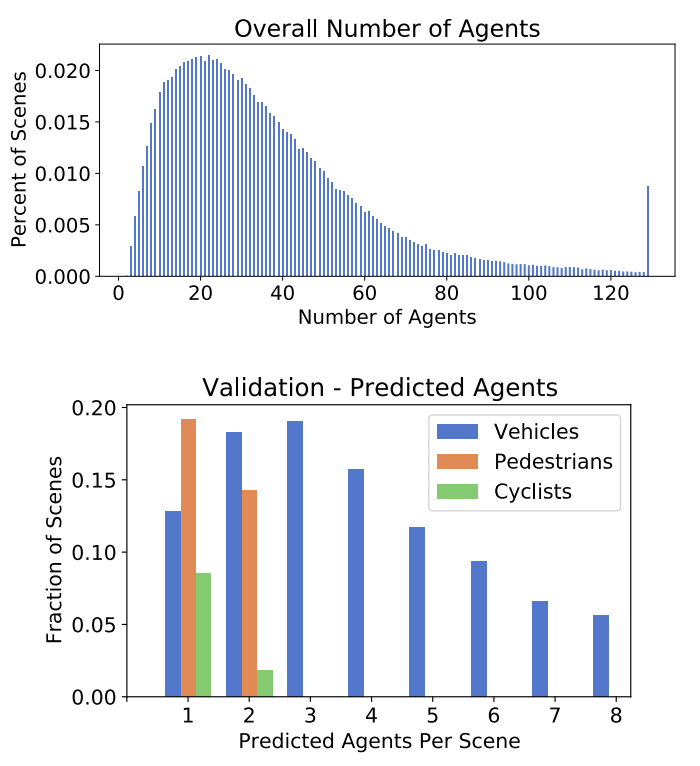
\includegraphics[width=0.9\textwidth]{Figures/Agents_Stat.png}
			\caption{The Waymo Open Motion Dataset(WOMD)\cite{Ettinger2021LargeSI} contains many agents including pedestrians and cyclists. Top: 46\% of scenes have more than 32 agents, and 11\% of scenes have more than 64
				agents. Bottom: In the standard validation set, 33.5\% of
				scenes require at least one pedestrian to be predicted, and
				10.4\% of scenes require at least one cyclist to be predicted.}
			\label{fig:Dataset1}
		\end{figure}
		
		\item Trajectories and Maximum Speed Analysis
		\begin{figure}[!htbp]
			\centering
			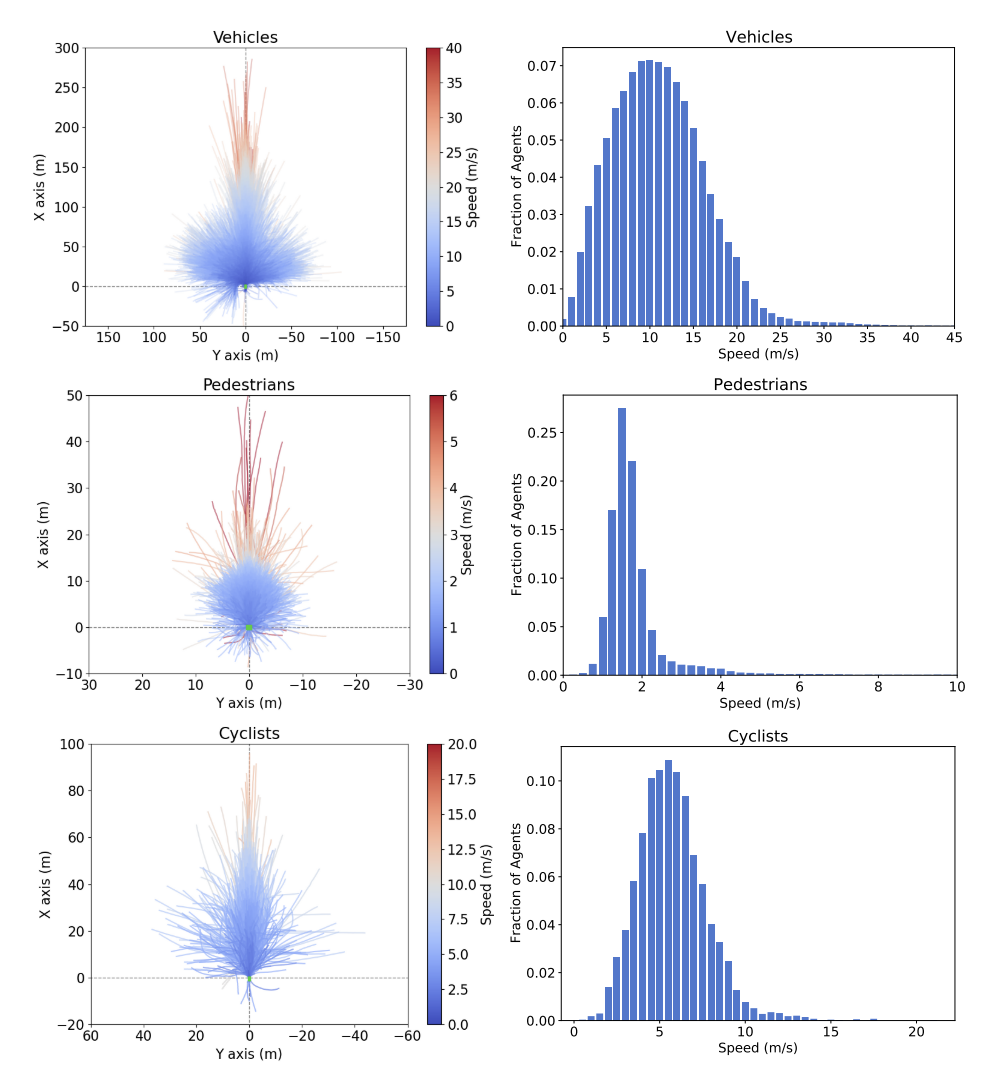
\includegraphics[width=0.9\textwidth]{Figures/Agents_Trajectories.png}
			\caption{Agents selected to be predicted have diverse
				trajectories. Left: Ground truth trajectory of each pre-
				dicted agent in a frame of reference where all agents start
				at the origin with heading pointing along the positive X
				axis (pointing up). Right: Distribution of maximum speeds
				achieved by all of the agents along their 9 second trajectory.
				Plots depict variety in trajectory shapes and speed profiles.}
			\label{fig:Dataset1}
		\end{figure}
	\end{enumerate}
	
\end{document}